%!TEX root = thesis.tex

\chapter{Introduction}
\label{ch:introduction}

\begin{wrapfigure}{r}{0.5\textwidth}
    \begin{center}
      
\includegraphics[width=0.5\textwidth]{images/pikachu.png}
    \end{center}
    \caption{Pikachu, one of the most popular Pokémon~\autocite{Fandom:AshsPikachu}}
    \label{fig:pikachu-image}
\end{wrapfigure}
Pokémon (an abbreviation for \textbf{Pocket Monsters}) is a media franchise managed by \textit{The Pokémon Company}, a company
founded by \textit{Nintendo}, \textit{Game Freak} and \textit{Creatures}~\autocite{Wikipedia:Pokemon}. Figure \ref{fig:pikachu-image} shows an image of
\textit{Pikachu}, one of the most popular Pokémon. Among multiple movies and series, a large variety of Pokémon games was released, starting with
\textit{Pokémon Red} and \textit{Pokémon Blue} which were released on 28. September 1998, also known as \ac{GEN1}-games. In order to promote
trading between players, \textit{Nintendo} published two very similar games at the same time. 
Both releases differ in the available Pokémon and some minor changes to the story. Therefore, in order to collect all available Pokémon,
players either had to buy two copies of the game or trade with a player that owns the counterpart. As of writing, there are eight major
releases, also called \textit{mainline games} with the latest being \textit{Pokémon Sword} and \textit{Pokémon Shield}. While the graphics
evolved a lot over the years (see figures \ref{fig:screenshot-red} and \ref{fig:screenshot-sword}), the key concept of the 
game remained mostly unchanged. 
\begin{figure}[ht]
  \centering
  \begin{minipage}{.5\textwidth}
    \centering
    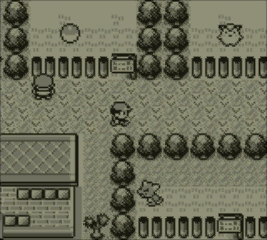
\includegraphics[width=.95\linewidth]{images/Red-0.jpg}
    \captionsetup{margin=0.5cm}
    \captionof{figure}*{Exploring the map}
  \end{minipage}%
  \begin{minipage}{.5\textwidth}
    \centering
    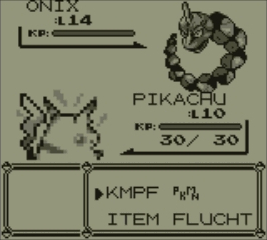
\includegraphics[width=.95\linewidth]{images/Red-1.jpg}
    \captionsetup{margin=0.5cm}
    \captionof{figure}*{Fighting another trainer}
  \end{minipage}
  \captionsetup{justification=centering,margin=1cm}
  \caption{Screenshots of Pokémon Red, the earliest Pokémon game. The game was released in 1996 for the Game Boy and has since been re-released multiple times. 
  Image source:~\autocite{Nintendo:PokemonRed}}
  \label{fig:screenshot-red}
\end{figure}
The player starts his journey in his hometown to become the \textit{Pokémon Champion}, which is the highest known 
level of rank for a Pokémon trainer~\cite{Bulbapedia:Pokémon-Champion}. In order
to achieve this goal, the player has to catch wild Pokémon and use them to create a team of up to six individual 
Pokémon which he then trains to unleash their full potential. 
\begin{figure}
  \centering
  \begin{minipage}{.5\textwidth}
    \centering
    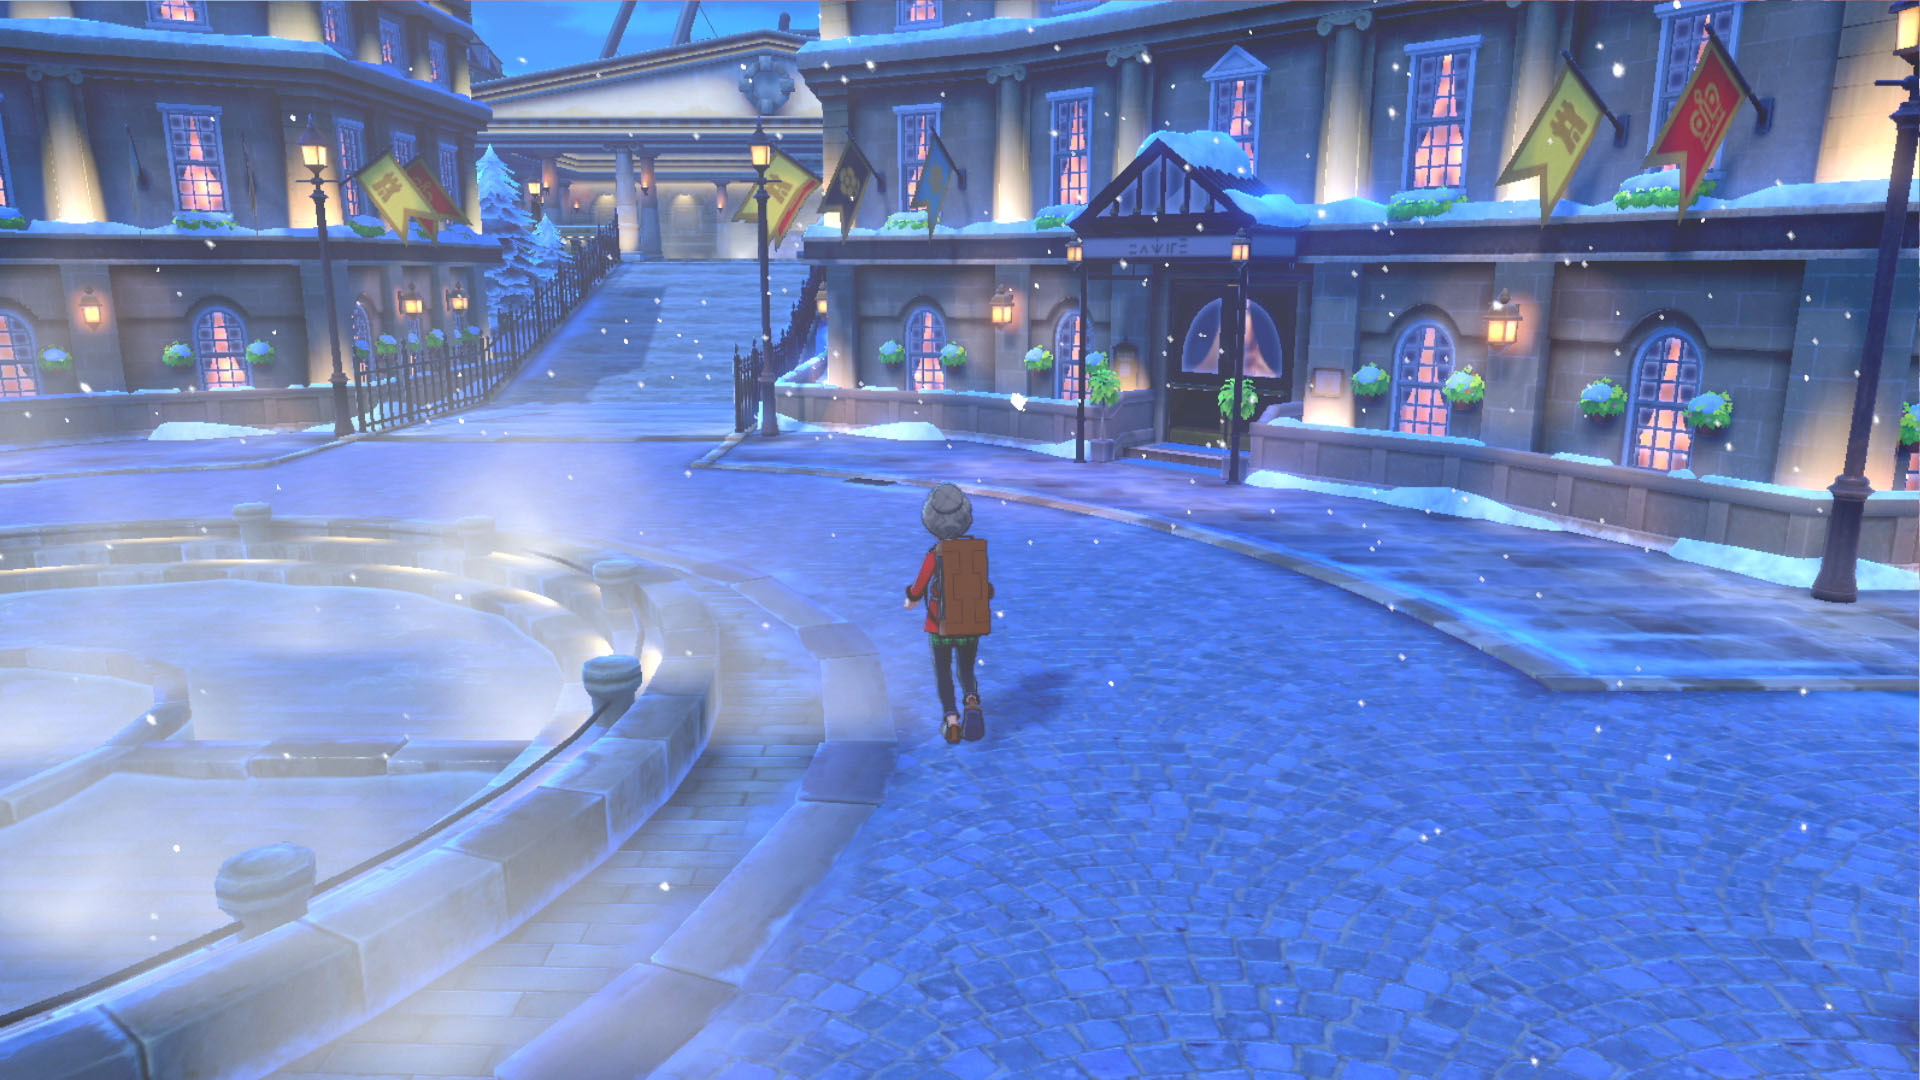
\includegraphics[width=.95\linewidth]{images/Sword-0.jpg}
    \captionsetup{margin=0.5cm}
    \captionof{figure}*{Exploring the map in Pokémon Sword.\\Image source:~\autocite{Pokemon:SwordMap}}
  \end{minipage}%
  \begin{minipage}{.5\textwidth}
    \centering
    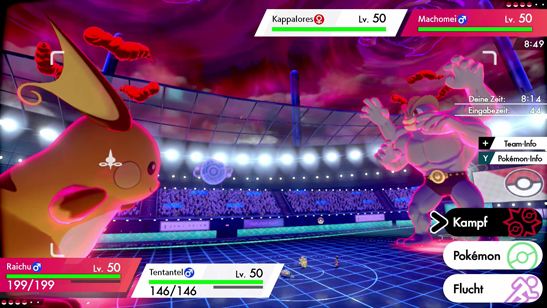
\includegraphics[width=.95\linewidth]{images/Sword-1.jpg}
    \captionsetup{margin=0.5cm}
    \captionof{figure}*{Fighting another trainer. \\Image source:~\autocite{Nintendo:PokemonSchwert}}
  \end{minipage}
  \caption{Screenshots of Pokémon Sword, the latest major Pokémon game released in 2019. While the graphics have 
  evolved, the core concept of the game, exploring and collecting Pokémon, remained the same.}
  \label{fig:screenshot-sword}
\end{figure}
This Thesis focuses exclusively on the battling aspect of the game as there are detailed lists of locations and
secrets there is to explore within the games. Pokémon battles are turn based where both players, unlike in 
for example chess, make their decisions at the same time. While the core battle mechanics are very simple, 
the game provides a lot of depth which led to the formation of a strong competitive battling scene.
As catching training Pokémon to a level where they are competitive viable is a time-intensive task, battle
simulators such as the open source project \textit{Pokémon Showdown}~\autocite{Showdown:Github} have arisen. On these fan made
platforms, players have access to all available Pokémon and can compete against each other in a large variety
of formats.
Figure \ref{fig:showdown-battle} shows a battle between two players on 
\textit{Pokémon Showdown}. The screenshot was taken from a \ac{GEN8} random battle between 
\textit{Buckfae} and another player\footnote{The other name was blurred}. The screenshot was taken
at the start of turn 19. Currently, the \textit{Mewtwo} of \textit{Buckfae} is at full health (indicated
red) while the opposing \textit{Kommo-o} has 33\% of \ac{HP} left. Below the avatars of both players,
the team is displayed, marked yellow for player two. While player one has three Pokémon remaining,
his opponent has four members alive. The Pokéball (bottom right) indicates a to the player unknown Pokémon.
Moreover, the blue box highlights the status modifications as well as boosts of the enemy Pokémon which will be
covered in section~\ref{sec:stat-calculation} and~\ref{sec:boosting} respectively.
Below the game window, the possible choices of the
player are displayed. \textit{Mewtwo} has access to the moves \textit{Fire Blast}, \textit{Recover}, \textit{Psystrike}
and \textit{Nastyplot}. In addition to \textit{Dynamaxing} which will be coverd in section~\ref{sec:dynamax} the player
also has the option to switch to either \textit{Sirfetch'd} or \textit{Vespiquen}. Lastly,
on the right-hand side a log of the previous turns can be found. In addition to the moves a Pokémon can use,
a Pokémon has one ability and can hold an item that yields advantages in battle. 
\\
Pokémon battles are simultaneous, meaning that both players move at the same time. Furthermore, each player has imperfect
information about the possible team of his opponent. 
Currently, there are approximately $7.9 \times 10^{44}$ 
(see section~\ref{sec:amout-states}) possible
starting positions for random battles which combined with the high dimensional feature vectors of states 
and the complex rules of the game result in Pokémon presenting an interesting challenge for AI to tackle. 
\\
This thesis gives an introduction to the main mechanics of the Pokémon genre while no prior knowledge of the 
game is required. 
Chapter \nameref{ch:relatedwork} introduces and compares different approaches and provides an in depth summarization
of the current state-of-the-art battling AI. 
Furthermore, an agent combining previously existing rule- and 
\textit{Minimax}-based implementations is developed to improve long term planning.
Challenges of evaluating Pokémon AI and the results of this research
are presented in \nameref{ch:evaluation}.